\chapter{SYSTEM DESIGN}

\section{Object-Oriented Design Approach}

\subsection{Refinement of Class, Object, State, Sequence and Activity Diagrams}

The final implementation follows the class structure identified during system analysis. The system is organized into service classes, adapter classes, routers, and utility modules. Abstract adapter classes provide common interfaces for embedding generation, vector database operations, and language model interaction, while concrete implementations such as \texttt{SentenceTransformersAdapter}, \texttt{QdrantAdapter}, and \texttt{GeminiAdapter} implement the required functionality. This modular design promotes extensibility and loose coupling. \par

The object design represents the runtime instantiation of the system components during execution. Service objects responsible for document ingestion, semantic retrieval, and response generation collaborate with instantiated adapter objects that manage embedding generation, vector database communication, and language model interaction. These runtime objects work together to process requests while maintaining clear separation of responsibilities. The object-oriented design enables efficient interaction among system components without introducing unnecessary dependencies. \par 

The runtime interactions remain consistent with the sequence diagrams developed during analysis. During document ingestion, uploaded PDFs are processed, chunked, embedded, and stored in Qdrant. During note generation, user requests are semantically matched with stored content before the retrieved context is provided to the Gemini language model for response generation. \par

The state design models the lifecycle of both document ingestion and note generation requests throughout system execution. Each process progresses through a series of well-defined states, beginning with request submission and concluding with either successful completion or error handling. State transitions occur based on the successful execution of each processing stage, ensuring that subsequent operations are performed only after the current state has been completed successfully. This design provides a structured approach to controlling the execution flow and managing exceptional conditions. \par

The activity design describes the workflows followed by the system while performing document ingestion and note generation. The activities are organized as sequential processing steps connected through decision points that determine the subsequent execution path based on validation results or runtime conditions. This workflow-oriented design clearly illustrates the operational logic of the system, simplifies the understanding of business processes, and facilitates future modifications by separating individual processing activities into well-defined functional steps. \par

\subsection{Component Diagram}
The Component Diagram illustrates the high-level software architecture of the proposed Academic Support System by depicting its major functional components and their dependencies. The system is organized into modular layers consisting of API routers, service modules, adapter modules, and external resources. The API routers receive client requests and delegate processing to the appropriate service modules. The service layer performs document ingestion, semantic retrieval, and response generation by utilizing the embedding, vector database, and language model adapters. The adapters provide a layer of abstraction for external technologies such as the Sentence Transformers embedding model, the Qdrant vector database, and the Gemini Large Language Model. This modular component-based architecture promotes maintainability, extensibility, and separation of concerns, allowing individual components to be modified or replaced without affecting the overall system. \par

% #NOTE figure here
\begin{figure}[H]
        \centering
    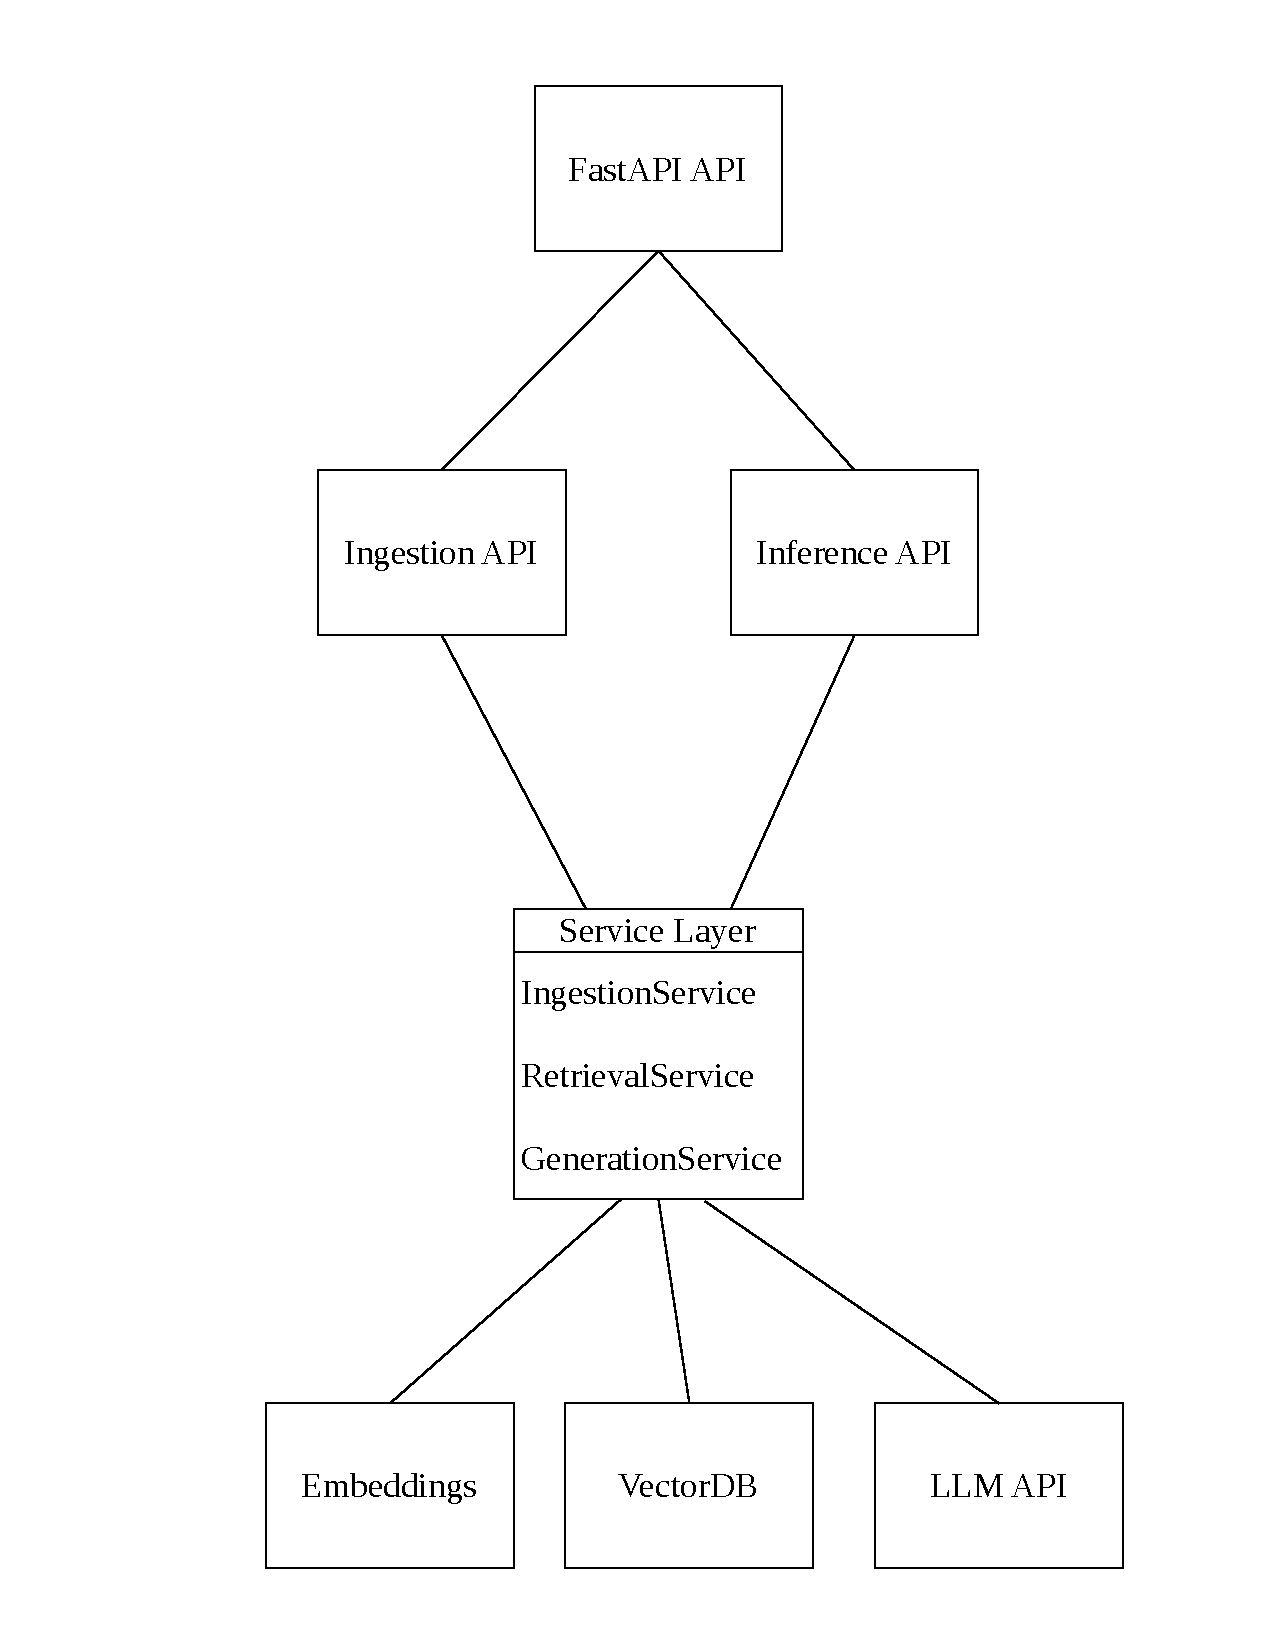
\includegraphics[
        % width=\linewidth,
        % height=0.95\textheight,
        % keepaspectratio,
        scale=0.3
        ]{figures/component-diagram.pdf}
    \caption{Component Diagram}
    \label{fig:component_diagram}
\end{figure}

\subsection{Deployment Diagram}
The Deployment Diagram illustrates the physical deployment architecture of the proposed Academic Support System. The system is designed as a client-server application in which client requests are sent to a locally hosted FastAPI backend server through HTTP. The backend hosts the API routers, business logic, and supporting service modules responsible for document ingestion and note generation. The server communicates with a cloud-based Qdrant vector database for storing and retrieving document embeddings, while response generation is performed by invoking the cloud-hosted Google Gemini API. This deployment architecture clearly separates the application logic, vector database, and external language model service, resulting in a scalable and modular system design. \par

%#NOTE - figure here
    \begin{figure}[H]
        \centering
    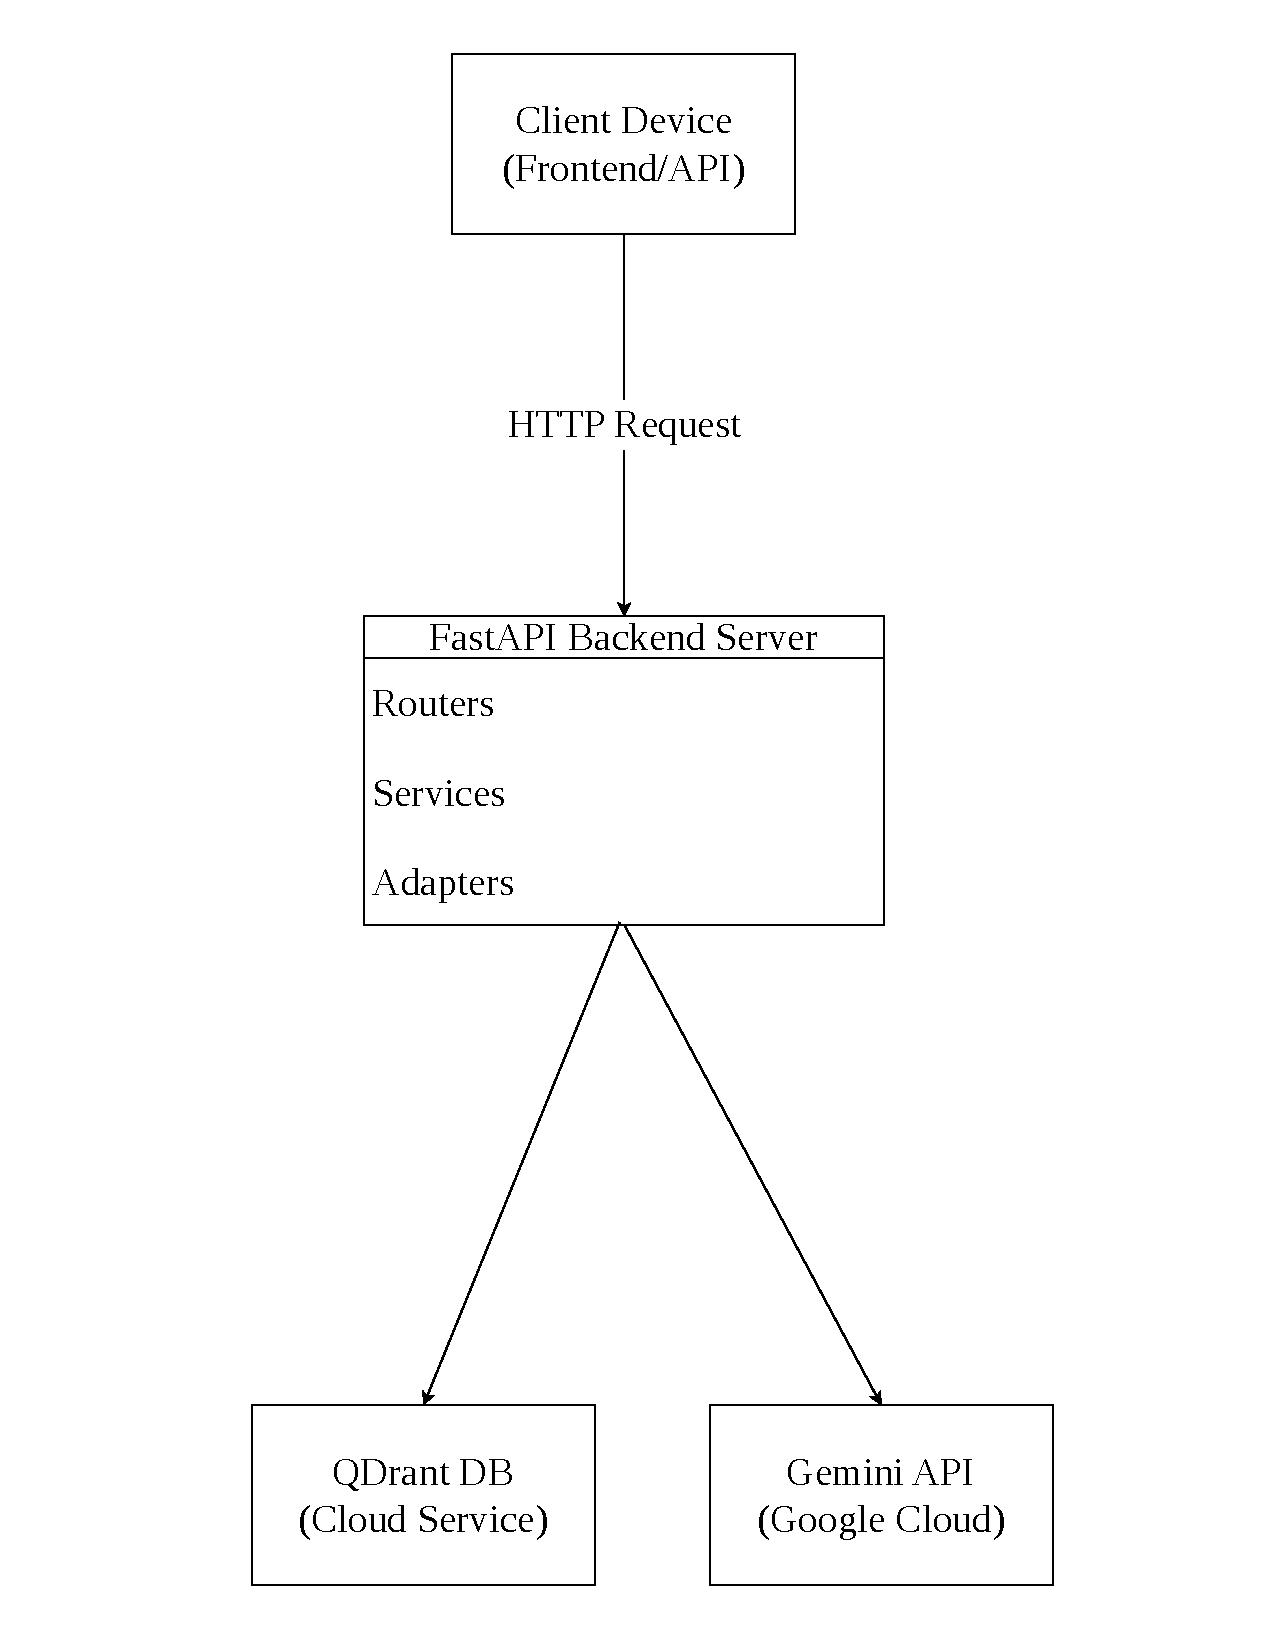
\includegraphics[
        % width=\linewidth,
        % height=0.95\textheight,
        % keepaspectratio,
        scale=0.3
        ]{figures/deployment-diagram.pdf}
    \caption{Deployment Diagram}
    \label{fig:deployment_diagram}
    \end{figure}

\section{Algorithm Details}

\begin{description}
    \item[Algorithm:] \textbf{Knowledge Base Creation}
    \item[Input:] Subject ID, Document ID, PDF document, metadata
    \item[Output:] Updated knowledge base
\end{description}

\begin{enumerate}
    \item Receive the uploaded PDF document and its associated metadata.
    \item Validate the uploaded document.
    \item Verify the provided metadata.
    \item If an existing knowledge base for the same document exists, remove the existing vectors from the database.
    \item Extract textual content from the PDF document.
    \item Divide the extracted text into smaller chunks.
    \item Generate vector embeddings for each text chunk.
    \item Store the embeddings together with their metadata in the Qdrant vector database.
    \item Return a success response.
    \item If any error occurs during processing, return an appropriate error response.
\end{enumerate}

\begin{description}
    \item[Algorithm:] \textbf{Note Generation using RAG}
    \item[Input:] Chapter/topic information and metadata
    \item[Output:] Generated academic notes
\end{description}
\begin{enumerate} 
    \item Receive the note generation request.
    \item Prepare the retrieval context from the request metadata.
    \item Generate an embedding for the requested topic.
    \item Retrieve the most relevant document chunks from the Qdrant vector database.
    \item Combine the retrieved context with the predefined prompt.
    \item. Send the constructed prompt to the Gemini Large Language Model.
    \item Receive the generated academic notes.
    \item Return the generated notes to the user.
    \item If any error occurs during retrieval or generation, return an appropriate error response.
\end{enumerate}